% \documentclass[12pt, twoside]{article}
\usepackage[letterpaper, margin=1in, headsep=0.2in]{geometry}
\setlength{\headheight}{0.6in}
%\usepackage[english]{babel}
\usepackage[utf8]{inputenc}
\usepackage{microtype}
\usepackage{amsmath}
\usepackage{amssymb}
%\usepackage{amsfonts}
\usepackage[nomessages]{fp} %\FPeval{\var-name}{2*sin(pi/6)}
\usepackage{siunitx} %units in math. eg 20\milli\meter
\usepackage{yhmath} % for arcs, overparenth command
\usepackage{tikz} %graphics
\usetikzlibrary{quotes, angles, arrows, arrows.meta}
\usepackage{graphicx} %consider setting \graphicspath{{images/}}
\usepackage{parskip} %no paragraph indent
\usepackage{enumitem}
\usepackage{multicol}
\usepackage{venndiagram}

\usepackage{fancyhdr}
\pagestyle{fancy}
\fancyhf{}
\renewcommand{\headrulewidth}{0pt} % disable the underline of the header
\raggedbottom
\hfuzz=2mm %suppresses overfull box warnings

\usepackage{hyperref}

\fancyhead[LE]{\thepage}
\fancyhead[RO]{\thepage \\ Name: \hspace{4cm} \,\\}
\fancyhead[LO]{BECA / Dr. Huson / Geometry\\*  Unit 1: Segments, length, and area\\* 12 Sept 2022}

\begin{document}

\subsubsection*{1.3 Homework: Vocabulary and segment addition}
\begin{enumerate}
\item Draw and label a line segment $\overline {AB}$ such that the distance between points $A$ and $B$ is 6 centimeters. \vspace{2cm}

\item Points that fall on the same straight line are $\rule{5cm}{0.15mm}$.

\item True or false: In mathematics we imagine that a straight line can go on forever in both directions. \bigskip

\item Use symbols to write the name of each geometric figure.
    \begin{enumerate}
    \begin{multicols}{3}
    \item
        \begin{tikzpicture}
        \draw [->, thick] (0,0)--(3,1.5);
        \draw [fill] (0,0) circle [radius=0.05] node[below]{$P$};
        \draw [fill] (2,1) circle [radius=0.05] node[below]{$Q$};
        \end{tikzpicture} \bigskip
    \item \hspace{1cm}
        \begin{tikzpicture}
        \draw [<->, thick] (1,0)--(1,3);
        \draw [fill] (1,0.5) circle [radius=0.05] node[right]{$N$};
        \draw [fill] (1,2.5) circle [radius=0.05] node[right]{$M$};
        \end{tikzpicture} \bigskip
    \item
      \begin{tikzpicture}
        \draw [-, thick] (1,0)--(0,2);
        \draw [fill] (1,0) circle [radius=0.05] node[below]{$G$};
        \draw [fill] (0,2) circle [radius=0.05] node[left]{$F$};
      \end{tikzpicture}
    \end{multicols}
    \end{enumerate} \vspace{1cm}

\item Given $\overline{ABC}$, $AB=2$, and $AC=12$. Mark the diagram, then find ${BC}$.\par \bigskip
\begin{tikzpicture}
  \draw [-, thick] (1,0)--(7,0);
  \draw [fill] (1,0) circle [radius=0.05] node[below]{$A$};
  \draw [fill] (2,0) circle [radius=0.05] node[below]{$B$};
  \draw [fill] (7,0) circle [radius=0.05] node[below]{$C$};
\end{tikzpicture} \vspace{2cm}

\item Two points $X(-2.8)$, $Y(5.1)$ are shown on the number line. \par \smallskip
\begin{tikzpicture}
    \draw[<->] (-3.5,0)--(6.5,0);
    \foreach \x in {-3,...,6}
        \draw[shift={(\x,0)}] (0pt,-3pt)--(0pt,3pt) node[below=5pt]{$\x$};
    \draw[fill] (-2.8,0) circle [radius=0.05] node[above]{$X$};
    \draw[fill] (5.1,0) circle [radius=0.05] node[above]{$Y$};
    \draw[thick] (-2.8,0)--(5.1,0);
\end{tikzpicture} \par \smallskip
Find the length of $\overline{XY}$. Show your work as an equation. 

\newpage
\item As shown, three collinear points with $LM=3x+4$, $MN=11$, $LN=33$. Find ${x}$.
    \begin{center}
    \begin{tikzpicture}
        \draw [-, thick] (0,0)--(9,0);
        \draw [fill] (0,0) circle [radius=0.05] node[below]{$L$};
        \draw [fill] (6,0) circle [radius=0.05] node[below]{$M$};
        \draw [fill] (9,0) circle [radius=0.05] node[below]{$N$};
        \node at (3,0) [above]{$3x+4$};
        \node at (7.5,0) [above]{$11$};
        \draw [<->, dashed] (0,-1)--(9,-1);
        \node at (4.5,-1) [below]{$33$};
    \end{tikzpicture}
    \end{center} \vspace{4cm}

\item Given $\overline{RST}$, $RS=3 \frac{2}{3}$, and $RT=9 \frac{1}{3}$. Find ${ST}$. (expressed as a fraction, not a decimal). \par \bigskip
    \begin{tikzpicture}
      \draw [-, thick] (0,0)--(7,0);
      \draw [fill] (0,0) circle [radius=0.05] node[below]{$R$};
      \draw [fill] (3,0) circle [radius=0.05] node[below]{$S$};
      \draw [fill] (7,0) circle [radius=0.05] node[below]{$T$};
    \end{tikzpicture} \vspace{2cm}

\item The diagram depicts a morning bicycle ride from home at 80th Street ($H$) to school at 164th Street ($S$) and an afternoon return from $S$ to $H$. \par \smallskip
    \begin{tikzpicture}[scale=0.12]
        \draw[<->] (66,0)--(184,0);
        \foreach \x in {70, 80,...,180}
            \draw[shift={(\x,0)}] (0pt,-16pt)--(0pt,16pt)node[below=5pt]{$\x$};
        \draw[fill] (80,0) circle [radius=0.3] node[above]{$H$};
        \draw[fill] (164,0) circle [radius=0.3] node[above]{$S$};
        \draw[thick] (80,0)--(164,0);
    \end{tikzpicture} 
    \begin{enumerate}[itemsep=1cm]
        \item Which ride is longer, the morning or afternoon? Or are they the same?
        \item In geometric notation, is there a difference between the segments $\overline{HS}$ and $\overline{SH}$?
    \end{enumerate} \vspace{1cm}

\item One day on Dr. Huson's commute straight north from 80th Street to 164th Street he realized he forgot something after riding ten blocks. So he had to ride back to his apartment before turning back around to ride to school as usual. How many total blocks did he ride that morning?


\end{enumerate}
\end{document}
